\documentclass[11pt, a4paper]{article}

\usepackage[english]{babel}
\usepackage{sleek}
\usepackage{common}

\title{Introduction to Artificial Intelligence (INFO8006)}
\subtitle{Exercise session 3}

\begin{document}

\maketitle

\begin{thbox}{Kolmogorov's axioms}
    A probability space is a sample space equipped with a probability function, i.e.
an assignment $P : \mathcal{P}(\Omega) \rightarrow \mathbb{R}$ such that
\begin{enumerate}
    \item $P(\omega) \in \mathbb{R}, 0 \leq P(\omega)$ for all $\omega \in \Omega$.
    \item $P(\Omega) = 1$.
    \item $P(\{\omega_1, ..., \omega_n\}) = \sum_{i=1}^n P(\omega_i)$.
\end{enumerate}
with $\Omega$ a \thighlight{sample space}, $\omega \in \Omega$ a \thighlight{sample point} and $\mathcal{P}(\Omega)$ the power set of $\Omega$.
\end{thbox}

\begin{thbox}{Probability rules}
    The \thighlight{product rule} states that
    $$
    P(a,b) = P(b)P(a\mid b) = P(a)P(b\mid a)
    $$ 
    from which \thighlight{Bayes' formula} is derived as
    $$
    P(a\mid b) = \dfrac{P(b\mid a)P(a)}{P(b)}
    $$
    with $P(a,b)$ being the joint probability of events $a$ and $b$, $P(b)$ - $P(a)$ the marginals and $P(a\mid b)$ - $P(b\mid a)$ the conditionals.\\

    The \thighlight{chain rule} states that 
    $$
    P(x_1,..,x_n) = \prod_{i=1}^n P(x_i\mid x_1, ..., x_{i-1}). 
    $$
\end{thbox}

\textbf{In session exercises:} Ex. 1, Ex. 2, Ex. 3, Ex. 5 

\newpage

\section{Beliefs}

Let $A$ and $B$ be two \emph{events} over the probability space $\Omega$. An agent holds the beliefs $P(A) = 0.4$ and $P(B) = 0.3$. What ranges of probabilities would it be rational for the agent to hold for the events $A \cup B$ and $A \cap B$ ? What if the agent also believes that $P(A | B) = 0.5$ ?

\begin{solution}
    \begin{enumerate}
        \item The agent's beliefs should satisfy
        \begin{alignat*}{2}
            0.4 = \max \cbk{P(A), P(B)} & \leq P(A \cup B) && \leq \min \cbk{1, P(A) + P(B)} = 0.7 \\
            0 = \max \cbk{0, P(A) + P(B) - 1} & \leq P(A \cap B) && \leq \min \cbk{P(A), P(B)} = 0.3 .
        \end{alignat*}
        This can be illustrated with Venn diagrams.

        \item If the agent believes that $P(A | B) = 0.5$, it should also believe that
        \begin{equation*}
            P(A \cap B) = P(A | B) P(B) = 0.5 \times 0.3 = 0.15,
        \end{equation*}
        thanks to Bayes rule. Then, the agent should rationally believe that
        \begin{equation*}
            P(A \cup B) = P(A) + P(B) - P(A \cap B) = 0.4 + 0.3 - 0.15 = 0.55.
        \end{equation*}
    \end{enumerate}
\end{solution}

\newpage

\section{(AIMA, Ex 13.8)}

\begin{table}[h]
    \centering
    \begin{tabular}{|c|c|c|c|c|}
        \hline
        & \multicolumn{2}{c|}{toothache} & \multicolumn{2}{c|}{no toothache} \\ \hline
        & catch & no catch & catch & no catch \\ \hline
        cavity & 0.108 & 0.012 & 0.072 & 0.008 \\ \hline
        no cavity & 0.016 & 0.064 & 0.144 & 0.576 \\ \hline
    \end{tabular}
\end{table}

Given the hereabove probability table, compute the following probabilities:

\begin{solution}
    In the following, we represent the events $toothache$, $catch$ and $cavity$ by the random variables $T, CT, CV: \Omega \mapsto \cbk{0, 1}$, respectively. Then, the hereabove table represents the joint probability distribution $P(T, CT, CV)$. When clear from context, we abbreviate the probability of a realization $(t, ct, cv)$ by $P(t, ct, cv)$ instead of $P(T = t, CT = ct, CV = cv)$.
\end{solution}

\begin{enumerate}
    \item $P(toothache)$

    \begin{solution}
        \begin{equation*}
            P(T = 1) = \sum_{ct} \sum_{cv} P(T = 1, ct, cv) = 0.108 + 0.012 + 0.016 + 0.064 = 0.2
        \end{equation*}
    \end{solution}

    \item $P(cavity)$

    \begin{solution}
        \begin{equation*}
            P(CV = 1) = \sum_{t} \sum_{ct} P(t, ct, CV = 1) = 0.108 + 0.012 + 0.072 + 0.008 = 0.2
        \end{equation*}
    \end{solution}

    \item $P(toothache | cavity)$

    \begin{solution}
        \begin{align*}
            P(T = 1 | CV = 1) = \frac{P(T = 1, CV = 1)}{P(CV = 1)} & = \frac{\sum_{ct} P(T = 1, ct, CV = 1)}{P(CV = 1)} \\
            & = \frac{0.108 + 0.012}{0.2} = 0.6
        \end{align*}
    \end{solution}

    \item $P(cavity | toothache \cup catch)$

    \begin{solution}
        \begin{align*}
            P(CV = 1 | T = 1 \cup CT = 1) & = \frac{P(T = 1 \cup CT = 1, CV = 1)}{P(T = 1 \cup CT = 1)} \\
            & = \frac{P(CV = 1) - P(T = 0, CT = 0, CV = 1)}{1 - P(T = 0, CT = 0)} \\
            & = \frac{0.2 - 0.008}{1 - 0.584} = \num{0.4615}
        \end{align*}
    \end{solution}

\end{enumerate}

\newpage

\section{(AIMA, Ex 13.15)}

After your yearly checkup, the doctor has bad news and good news. The bad news is that you tested positive for a serious disease and that the test is \qty{99}{\percent} accurate, \ie{} the probability of testing positive when you do have the disease is \num{0.99} and the probability of testing positive when you don't is \num{0.01}. The good news is that this is a rare disease, striking only 1 in \num{10000} people of your age. Why is it good news that the disease is rare? What are the chances that you actually have the disease?

\begin{solution}
    It is a good news because the conditional probability will drop due to the weak prior value. Indeed,
    \begin{align*}
        P(d | t) & = \frac{P(t | d) P(d)}{P(t)} \\
        & = \frac{P(t | d) P(d)}{P(t | d) P(d) + P(t | \neg d) P(\neg d)} \\
        & = \frac{0.99 \times \num{e-4}}{0.99 \times \num{e-4} + 0.01 \times (1 - \num{e-4})} = \num{0.0098} .
    \end{align*}
\end{solution}

\newpage

\section{(AIMA, Ex 13.13)}

For each of the following statements, either prove it is valid or give a counterexample.

\begin{enumerate}
    \item If $P(a | b, c) = P(b | a, c)$, then $P(a | c) = P(b | c)$.

    \begin{solution}
        True. By the conditional probability rule we have $P(a | b, c) P(b, c) = P(b | a, c) P(a, c)$, which by assumption reduces to $P(b, c) = P(a, c)$ and thereby $P(b | c) = P(a | c)$.
    \end{solution}

    \item If $P(a | b, c) = P(a)$, then $P(b | c) = P(b)$.

    \begin{solution}
        False. The statement $P(a | b, c) = P(a)$ merely states that $a$ is independent of $b$ and $c$, it makes no claim regarding the dependence of $b$ and $c$. Counterexample: $a$ and $b$ record the results of two independent coin flips, and $c = b$.
    \end{solution}

    \item If $P(a | b) = P(a)$, then $P(a | b, c) = P(a | c)$.

    \begin{solution}
        False. While the statement $P(a | b) = P(a)$ implies that $a$ is independent of $b$, it does not imply that $a$ is conditionally independent of $b$ given $c$. Counterexample: $a$ and $b$ record the results of two independent coin flips, and $c = a \vee b$.
    \end{solution}
\end{enumerate}

\newpage

\section{Bag of coins}

We have a bag of three biased coins $a$, $b$, and $c$ with probabilities of coming up heads of \qty{20}{\percent}, \qty{60}{\percent}, and \qty{80}{\percent}, respectively. One coin is drawn randomly from the bag (with equal probability of drawing each of the three coins), and then the coin is flipped three times to generate the outcomes $X_1$, $X_2$ and $X_3$ (heads or tail).

\begin{enumerate}
    \item Draw the Bayesian network corresponding to this setup and define the corresponding conditional probability tables (CPTs).

    \begin{solution}
        The process is described with the following random variables:
        \begin{itemize}
            \item $Y \in \cbk{a, b, c}$, the coin drawn from the bag.
            \item $X_i \in \cbk{h, t}$, the realization of the $i$-th coin toss.
        \end{itemize}
        The variable $Y$ is the parent of $X_i$, it should be put before in the network ordering.

        \begin{figure}[h]
            \begin{subfigure}[c]{0.495\textwidth}
                \centering
                \begin{tikzpicture}[node distance = 2cm]
                    \node[state] (Y) {$Y$};
                    \node[state] (X1) [below left of=Y] {$X_1$};
                    \node[state] (X2) [below of=Y] {$X_2$};
                    \node[state] (X3) [below right of=Y] {$X_3$};

                    \draw[arrow] (Y) to (X1);
                    \draw[arrow] (Y) to (X2);
                    \draw[arrow] (Y) to (X3);
                \end{tikzpicture}
            \end{subfigure}
            \begin{subfigure}[c]{0.495\textwidth}
                \centering
                \begin{tabular}{c|cc}
                    \toprule
                     $Y$ & $P(Y)$ & $P(X_i = h | Y)$ \\
                     \midrule
                     $a$ & $\frac{1}{3}$ & $0.2$ \\
                     $b$ & $\frac{1}{3}$ & $0.6$ \\
                     $c$ & $\frac{1}{3}$ & $0.8$ \\
                    \bottomrule
                \end{tabular}
            \end{subfigure}
        \end{figure}
    \end{solution}

    \item Determine which coin ($a$, $b$ or $c$) is most likely to have been drawn from the bag if the observed tosses came out heads twice and tail once.

    \begin{solution}
        In order to find the most likely coin, we have to calculate the conditional probability distribution $P(Y | X_1 = h, X_2 = h, X_3 = t)$\footnote{It should be noted that the order of the tosses is irrelevant as they are performed independently.}. Thanks to Bayes rule, we have
        \begin{equation*}
        P(Y | X_1 = h, X_2 = h, X_3 = t) = \alpha P(X_1 = h, X_2 = h, X_3 = t | Y) P(Y).
        \end{equation*}
        But we know that $X_1$, $X_2$ and $X_3$ are independent with respect to $Y$, meaning that
        \begin{equation*}
            P(X_1, X_2, X_3 | Y) = P(X_1 | Y) P(X_2 | Y) P(X_3 | Y).
        \end{equation*}
        Then, we have
        \begin{equation*}
            P(Y | X_1 = h, X_2 = h, X_3 = t) = \alpha \times \frac{1}{3} \times \begin{cases}
                0.2 \times 0.2 \times 0.8 = \num{0.032} & \text{if } Y = a \\
                0.6 \times 0.6 \times 0.4 = \num{0.144} & \text{if } Y = b \\
                0.8 \times 0.8 \times 0.2 = \num{0.128} & \text{if } Y = c \\
            \end{cases}
        \end{equation*}
        meaning that $b$ is the most likely coin to have been drawn. Interestingly, we don't need to normalize the distribution as we only care about the maximum.
    \end{solution}
\end{enumerate}

\newpage

\section{Handedness (AIMA, Ex 14.6)}

Let $H_x$ be a random variable denoting the handedness of an individual $x$, with possible values $l$ or $r$. A common \emph{hypothesis} is that left or right-handedness is inherited by a simple mechanism; that is, there is a gene $G_x$, also with values $l$ or $r$, and $H_x$ turns out the same as $G_x$ with some probability $s$.

Furthermore, the gene itself is equally likely to be inherited from either of the individual's parents, with a small nonzero probability $m$ of a random mutation flipping the gene.

\begin{enumerate}
    \item Which of the following networks claim that $P(G_{child} | G_{mother}, G_{father}) = P(G_{child})$ ?

    \begin{figure}[h]
        \centering
        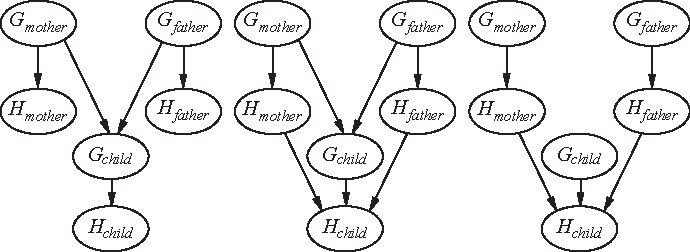
\includegraphics[width=0.9\textwidth]{figures/e3_handedness.pdf}
    \end{figure}

    \begin{solution}
        The third one, as the node $G_{child}$ does not have any parents.
    \end{solution}

    \item Which of the networks make independence claims that are consistent with the hypothesis about the inheritance of handedness ?

    \begin{solution}
        The first and second ones. It should be noted that the second one is also valid as it makes \emph{less} assumptions about the variables dependencies, \ie{} it is more general than the first one.
    \end{solution}

    \item Write down the CPT for the $G_{child}$ nodes in first network, in terms of $s$ and $m$.

    \begin{solution}
        \begin{table}[h]
            \centering
            \begin{tabular}{cc|c}
                \toprule
                 $G_{mother}$ & $G_{father}$ & $P(G_{child} = l | G_{mother}, G_{father})$ \\
                 \midrule
                 $l$ & $l$ & $1 - m$ \\
                 $l$ & $r$ & $0.5$ \\
                 $r$ & $l$ & $0.5$ \\
                 $r$ & $r$ & $m$ \\
                \bottomrule
            \end{tabular}
        \end{table}
    \end{solution}

    \item Suppose that $P(G_{mother} = l) = P(G_{father} = l) = q$. In the first network, derive an expression for $P(G_{child} = l)$ in terms of $s$, $m$ and $q$.
    \begin{solution}
        \begin{align*}
            P(G_{child} = l) & = \sum_{g_m} \sum_{g_f} P(G_{child} = l, g_m, g_f) \\
            & = \sum_{g_m} \sum_{g_f} P(G_{child} = l | g_m, g_f) P(g_m) P(g_f) \\
            & = (1 - m) q^2 + 0.5 (1 - q) q + 0.5 q (1 - q) + m (1 - q)^2 \\
            & = q + m - 2qm
        \end{align*}
    \end{solution}

    \item Under conditions of genetic equilibrium, we expect the distribution of genes to be the same across generations. Use this to calculate the value of $q$, and, given what you know about handedness in humans, explain why the hypothesis described at the beginning of this question must be wrong.

    \begin{solution}
        Under genetic equilibrium, we have $P(G_{child} = l) = P(G_{parent} = l) = q$. Therefore, $q = q + m - 2 q m$ meaning that $q = 0.5$. In practice, being left-handed is much more rare than being right-handed which invalidates the initial hypothesis.
    \end{solution}
\end{enumerate}

\newpage

\startquiz

The Bayes’ rule states that ...
\begin{itemize}
    \item $P(x\mid y) = \frac{P(y\mid x)P(y)}{P(x)}$.
    \solitem $P(x\mid y) = \frac{P(y\mid x)P(x)}{P(y)}$.
    \item $P(y\mid x) = \frac{P(x\mid y)P(x)}{P(y)}$.
    \item $P(x) = \frac{P(x\mid y)P(y)}{P(x)}$.
\end{itemize}

Which of the following is true?
\begin{itemize}
    \item $P(x, y \mid z) = \frac{P(x \mid y,z)}{P(y,z \mid x)}$.
    \item $P(x, y, z) = P(x)P(y)P(z)$.
    \solitem $P(x, y \mid z) = P(y\mid x,z)P(x\mid z)$. 
    \item $P(x\mid y,z) = \frac{P(x,y,z)}{P(y)P(z)}$.
\end{itemize}

Naive Bayes model assumes ... 
\begin{itemize}
    \solitem pairwise conditional independence between effects given the cause.
    \item pairwise independence between effects.
    \item independence between effects and cause.
    \item conditional independence between each effect and the cause, given another effect.
\end{itemize}

The Bayes' rule can be read as "The posterior is equal to ... 
\begin{itemize}
    \item the product of the likelihood and the prior".
    \item the ratio between the posterior distribution and the evidence, times the prior".
    \item the likelihood to prior ratio multiplied by the evidence".
    \solitem the likelihood to evidence ratio multiplied by the prior".
\end{itemize}

\end{document}